\chapter{Algorithm description \todo{To be renamed?}}

Electron backscatter diffraction (EBSD) is a scientific tool used to examine crystalline materials. The principle of EBSD is sketched in \cref{ebsd-principle}. It is based on electron diffraction: when a beam of electrons is emitted towards the specimen, some of the electrons backscatter. They are then reflected on phosphor screen which is coupled with compact lens that directs the captured image towards a camera. The result of this procedure is a grayscale image of the \emph{electron backscatter pattern} (EBSP). An example of EBSP is shown in \cref{roi-shifts:initial}.

\begin{figure}
	\centering
	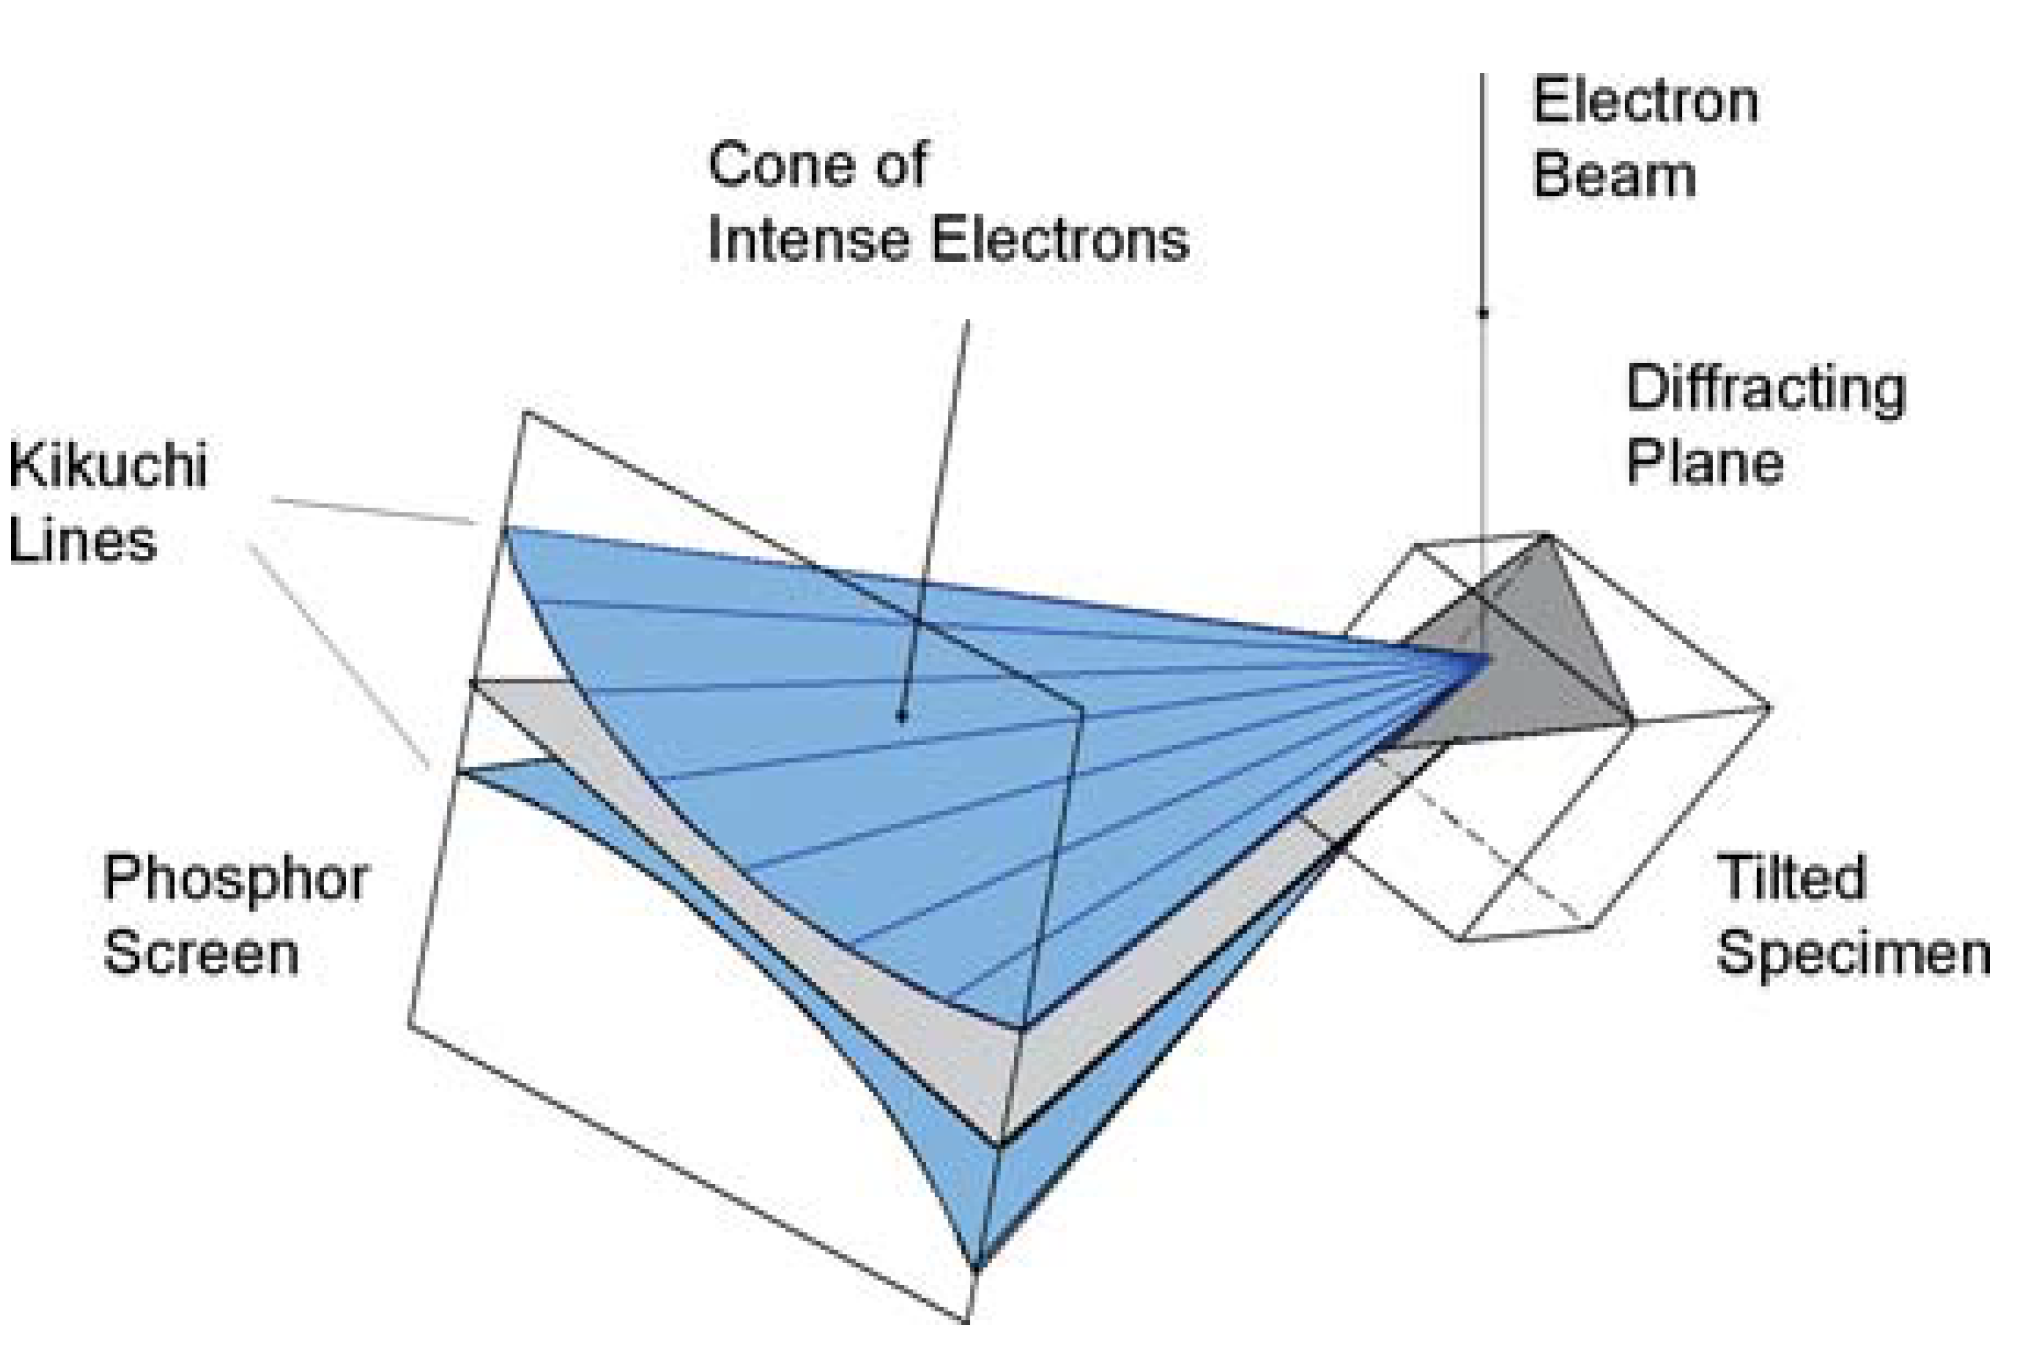
\includegraphics[width=0.7\textwidth]{img/ebsd_principle}
	\caption{The principle of EBSD. The image is taken from \cite{schwartz2009electron}.}
	\label{ebsd-principle}
\end{figure}

%\begin{figure}
%	\centering
%	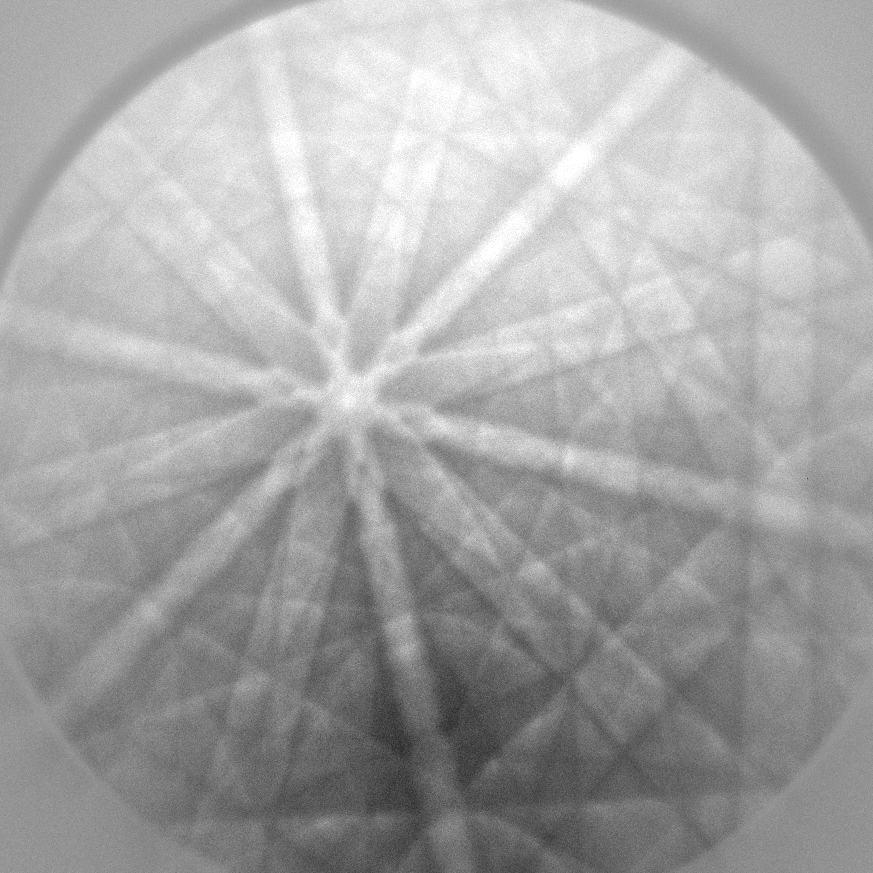
\includegraphics[width=0.7\textwidth]{img/INITIAL_x0y0}
%	\caption{Electron backscatter pattern of the FeAl compound.}
%	\label{ebsp-example}
%\end{figure}

The electrons do not reflect randomly, but based on the examined specimen, they backscatter in a specific way, forming \emph{Kukuchi lines} observable in the EBSP. The geometry of Kukuchi lines can be interpreted as a projection of the specimen crystal structure on the flat phosphor screen.

EBSD is commonly used with scanning electron microscopes (SEM). A SEM is a device that repeatedly emits an electron beam towards the specimen, scanning the surface in a raster pattern. That allows to create images of the surface of the sample with much greater magnification than light microscopes.

When used with EBSD, it creates the EBSPs in a raster scan pattern. It scans a part of the surface, measuring the crystalline structure of the specimen in many spots and saving the information as an EBSP. So the procedure results in thousands of images, one for each point in the raster. For example, test data that we used for this thesis contained over 15000 images taken from a 120x120 raster covering an area of the specimen surface approximately \SI{70}{\nano\meter}~x~\SI{70}{\nano\meter} big.

When the crystal structure of material is changed (e.g. under stress), the deformation can be observed in the EBSP too. Therefore, EBSPs of deformed specimen can be compared to undeformed ones to measure elastic strain and crystal lattice rotation.  \Cref{roi-shifts} shows a visualization of such comparison. Since different parts of the images may be deformed differently, a commonly used technique \cite{wilkinson2006high,wilkinson2010high,britton2012high} is to choose several (usually tens to hundreds) subregions of the EBSPs and determine the vector of shift between the corresponding regions from both patterns. The shifts estimate the real deformation of the crystalline structure.

\begin{figure}
	
	\begin{subfigure}{.4\textwidth}
		\centering
		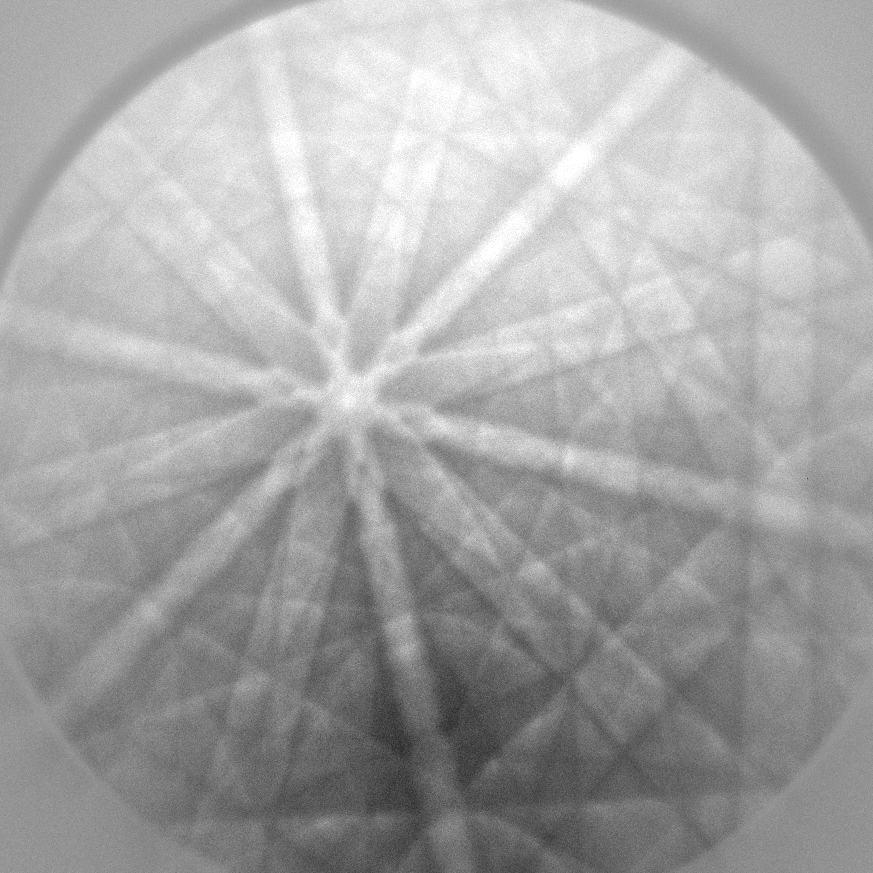
\includegraphics[width=.9\linewidth]{img/roi_shifts_initial}
		\caption{Initial, undeformed pattern}
		\label{roi-shifts:initial}
	\end{subfigure}%
	\begin{subfigure}{.4\textwidth}
		\centering
		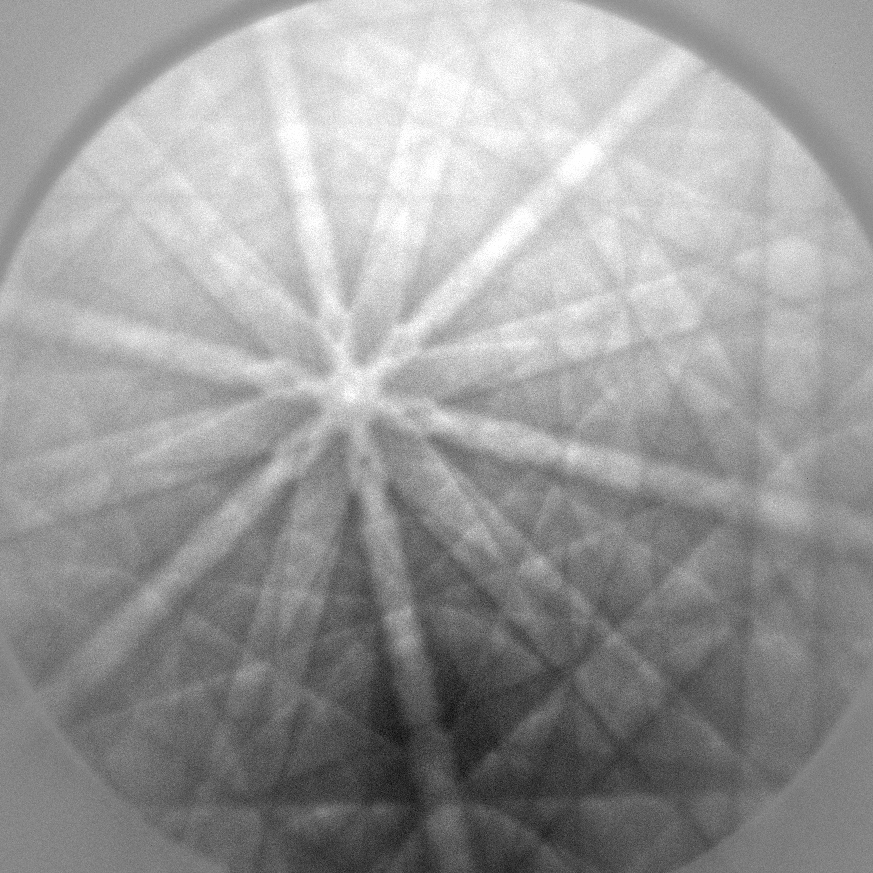
\includegraphics[width=.9\linewidth]{img/DEFORMED_x3600y6235}
		\caption{Deformed pattern}
		\label{fig:sub2}
	\end{subfigure}
	\centering
	\begin{subfigure}{.4\textwidth}
		\centering
		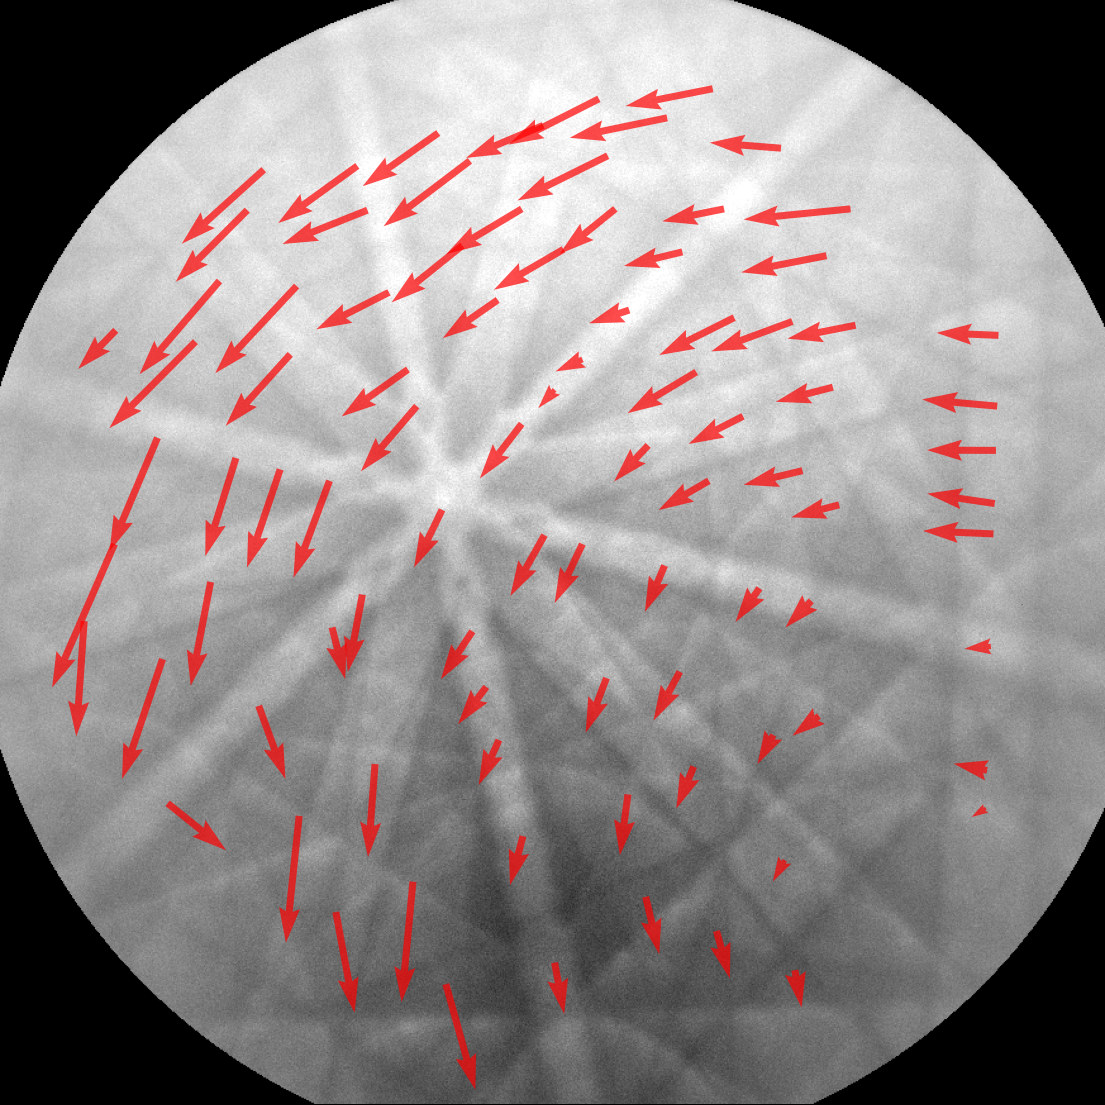
\includegraphics[width=.9\linewidth]{img/roi_shifts}
		\caption{Deformation visualization}
		\label{fig:sub2}
	\end{subfigure}

	\caption{Deformed pattern with arrows visualizing the deformation. The arrows are upscaled for the visualization, because the pattern is deformed only by several pixels (the biggest offset is less than 10 pixels long).}
	\label{roi-shifts}
\end{figure}

The comparison is done by cross correlating respective subregions of the deformed and reference EBSPs. The position of the maximum value in the correlation result determines the most probable shift with one pixel precision, which is not enough. To achieve subpixel accuracy, we estimate the peak of the cross correlation by interpolating from a small neighborhood of the maximum.

Once the shifts are computed, they are further processed to obtain an estimation of the actual crystal deformation and other characteristics. However, we do not address that part of the analysis in this thesis, as it is not nearly as computationally expensive as the cross correlation of the EBSPs. Moreover, the comparison is commonly used in analysis of EBSPs, while the processing of the shifts may be different for various purposes.

In this chapter we describe the technique based on cross correlation in detail.
\todo{summarize the chapter once it is done}

\section{Cross correlation}

Cross correlation provides a measure of similarity of two series for each possible shift between them. It is used in signal processing to find a shorter known feature in a signal or in image processing to locate a smaller shape in a bigger picture. In analysis of EBSPs, it is used to find the most probable relative displacement between two images (subregions of images).

Cross correlation of two discrete functions $f$ and $g$ is function $C$ defined as follows:
$$
C[n] = (f \star g)[n] = \sum_{m=-\infty}^{\infty}f[m]g[m+n],
$$
where $\star$ denotes cross correlation.

If $C = f \star g$ then $C[n]$ is a number that tells us how much are functions $f$ and $g$ similar, when $g$ is shifted by $n$ to the left. For each negative $n$, $g$ is shifted to the right. \Cref{correlation-example} shows two example functions and their cross correlation.

\begin{figure}
	\centering
	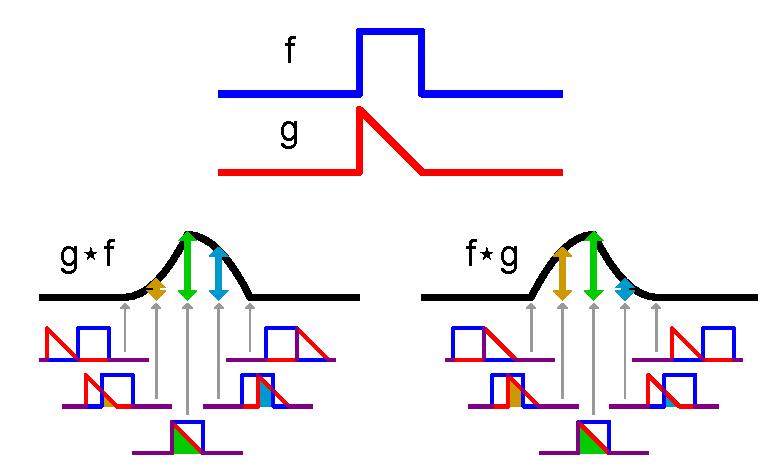
\includegraphics[width=0.7\linewidth]{img/correlation}
	\caption{The principle of EBSD. The image is taken from \cite{correlation_example}.}
	\label{correlation-example}
\end{figure}

Definition of cross correlation can be extended for two dimensions. For two two--dimensional functions $f$ and $g$, their cross correlation is defined as:
$$
C[i,j] = (f \star g)[i,j] = \sum_{n=-\infty}^{\infty}\sum_{m=-\infty}^{\infty}f[n,m]g[n+i,m+j].
$$

Analogously to one--dimensional cross correlation, $(f \star g)[i,j]$ is a number that is higher if $f$ is similar to $g$ shifted by $i$ horizontally and by $j$ vertically. \Cref{2d-correlation-example} demonstrates how cross correlation can be used to search for a smaller pattern in a bigger picture. The brightest points (maxima) in \cref{2d-correlation-example-result} correspond to the best matches between the pattern and the image.

\begin{figure}
	\centering
		\begin{subfigure}{.4\textwidth}
		\centering
		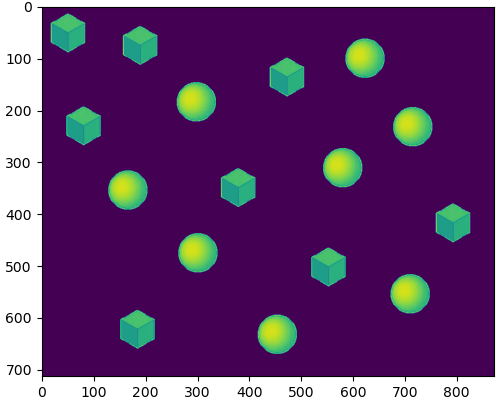
\includegraphics[width=\linewidth]{img/shapes}
		\caption{An image}
		\label{roi-shifts:initial}
	\end{subfigure}
	\begin{subfigure}{.4\textwidth}
	\centering
	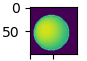
\includegraphics[width=0.4\linewidth]{img/search_shape}
	\caption{Search pattern}
	\label{fig:sub2}
	\end{subfigure}
	\begin{subfigure}{.5\textwidth}
		\centering
		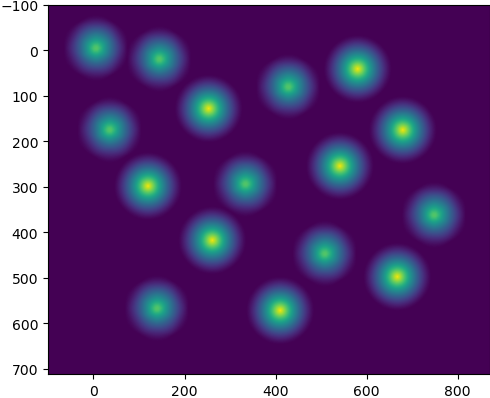
\includegraphics[width=\linewidth]{img/shapes_correlated}
		\caption{Cross correlation of the (a) and (b) images}
		\label{2d-correlation-example-result}
	\end{subfigure}
	
	\caption{The principle of EBSD. The image is taken from \cite{correlation_example}.}
	\label{2d-correlation-example}
\end{figure}

Theoretically, the domain of cross correlation is whole $\mathbb{Z}^2$. However, when cross correlating two images, $(f \star g)[i,j]$ does not make sense for too big $i$ or $j$ because the images would be shifted so much they would not overlap. For two images with sizes $w_1 \times h_1$ and $w_2 \times h_2$, the size of their cross correlation is $(w_1 + w_2 - 1) \times (h_1 + h_2 - 1)$. The result is a rectangle with the following corners: $[-w_1+1,-h_1+1]$, $[-w_1+1,h_2-1]$, $[w_2-1,h_2-1]$, $[w_2-1,-h_1+1]$. Those are the points of cross correlation, where the result is computed from the images overlapping only by one pixel.

\subsection{Normalized cross correlation}

Cross correlation as it is defined in the previous section has a major flaw for image processing: it is affected by the brightness of the images.


\begin{figure}
	\centering
	\begin{subfigure}{.4\textwidth}
		\centering
		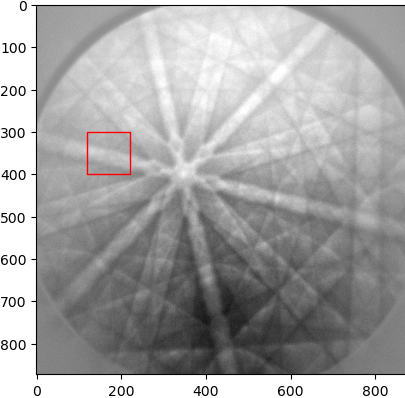
\includegraphics[width=\linewidth]{img/normalized_initial}
		\caption{An image}
		\label{roi-shifts:initial}
	\end{subfigure}
	\begin{subfigure}{.4\textwidth}
		\centering
		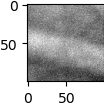
\includegraphics[width=0.4\linewidth]{img/normalized_pattern}
		\caption{Search pattern}
		\label{fig:sub2}
	\end{subfigure}
	\begin{subfigure}{.49\textwidth}
		\centering
		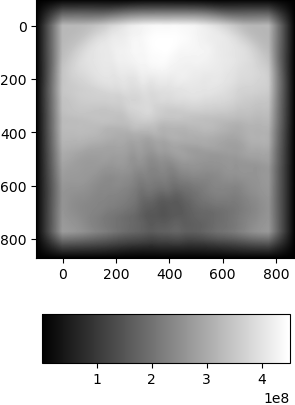
\includegraphics[width=\linewidth]{img/normalized_simple_corr}
		\caption{Simple cross correlation of the (a) and (b) images}
		\label{2d-correlation-example-result}
	\end{subfigure}
	\begin{subfigure}{.49\textwidth}
		\centering
		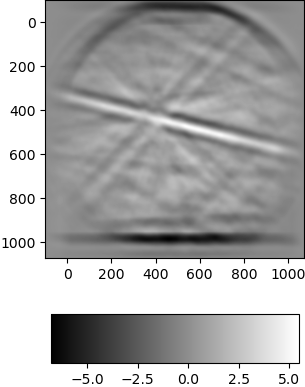
\includegraphics[width=\linewidth]{img/normalized_corr}
		\caption{Normalized cross correlation of the (a) and (b) images}
		\label{2d-correlation-example-result}
	\end{subfigure}
	
	\caption{The principle of EBSD. The image is taken from \cite{correlation_example}.}
	\label{2d-correlation-example}
\end{figure}


\section{Algorithm description}



\begin{algorithm}
	\caption{EBSP deformation processing}
	
	\KwIn{
		one reference EBSP\;
		N deformed EBSPs\;
	 	position of M regions of interest (ROI) from each EBSP to be compared \;
 		size of one ROI\;}
	\KwOut{deformation shifts for all M ROIs from all N deformed EBSPs}
	\vspace{5px}
	
	refEBSP  $\leftarrow$ load reference EBSP from disk\;
	\ForEach{deformed EBSP}{
		defEBSP $\leftarrow$ load EBSP from disk\;
		\ForEach{ROI in EBSP}{
			refROI, defROI $\leftarrow$ extract ROI from refEBSP and defEBSP\;
			
			find the mean of both ROIs and subtract it\;
			apply (Hann) window to both ROIs
			
			crossResult $\leftarrow$ cross correlate refROI with defROI\;
			%
			maxX, maxY $\leftarrow$ subpixelPeak(crossResult)\;
			output [maxX, MaxY]\;
		}
	}
	
	\SetKwProg{Fn}{Function}{ is}{end}
	\SetKwFunction{FSubpixelPeak}{subpixelPeak}    
	\Fn{\FSubpixelPeak{crossResult}}{
		max $\leftarrow$ argmax(crossResult)\;
		neigh $\leftarrow$ extract neighborhood of max\;
		
		fit a quadratic function to neigh using the least squares method\;
		\KwRet maximum of the quadratic function\;
	}
	
	
\end{algorithm}

